\chapter{Matter and Energy}

The universe is made of matter and energy. Current models posit that the universe
is approximately 68\% dark energy, 27\% dark matter, and 5\% ordinary matter. 
Everything you can see and touch is part of the small part of the universe made 
of ordinary matter. Most science deals with ordinary matter and its interactions; 
highly trained theoretical physicists are currently debating the nature and 
effects of dark matter and dark energy. 
\begin{wrapfigure}{r}{2.5in}
\noindent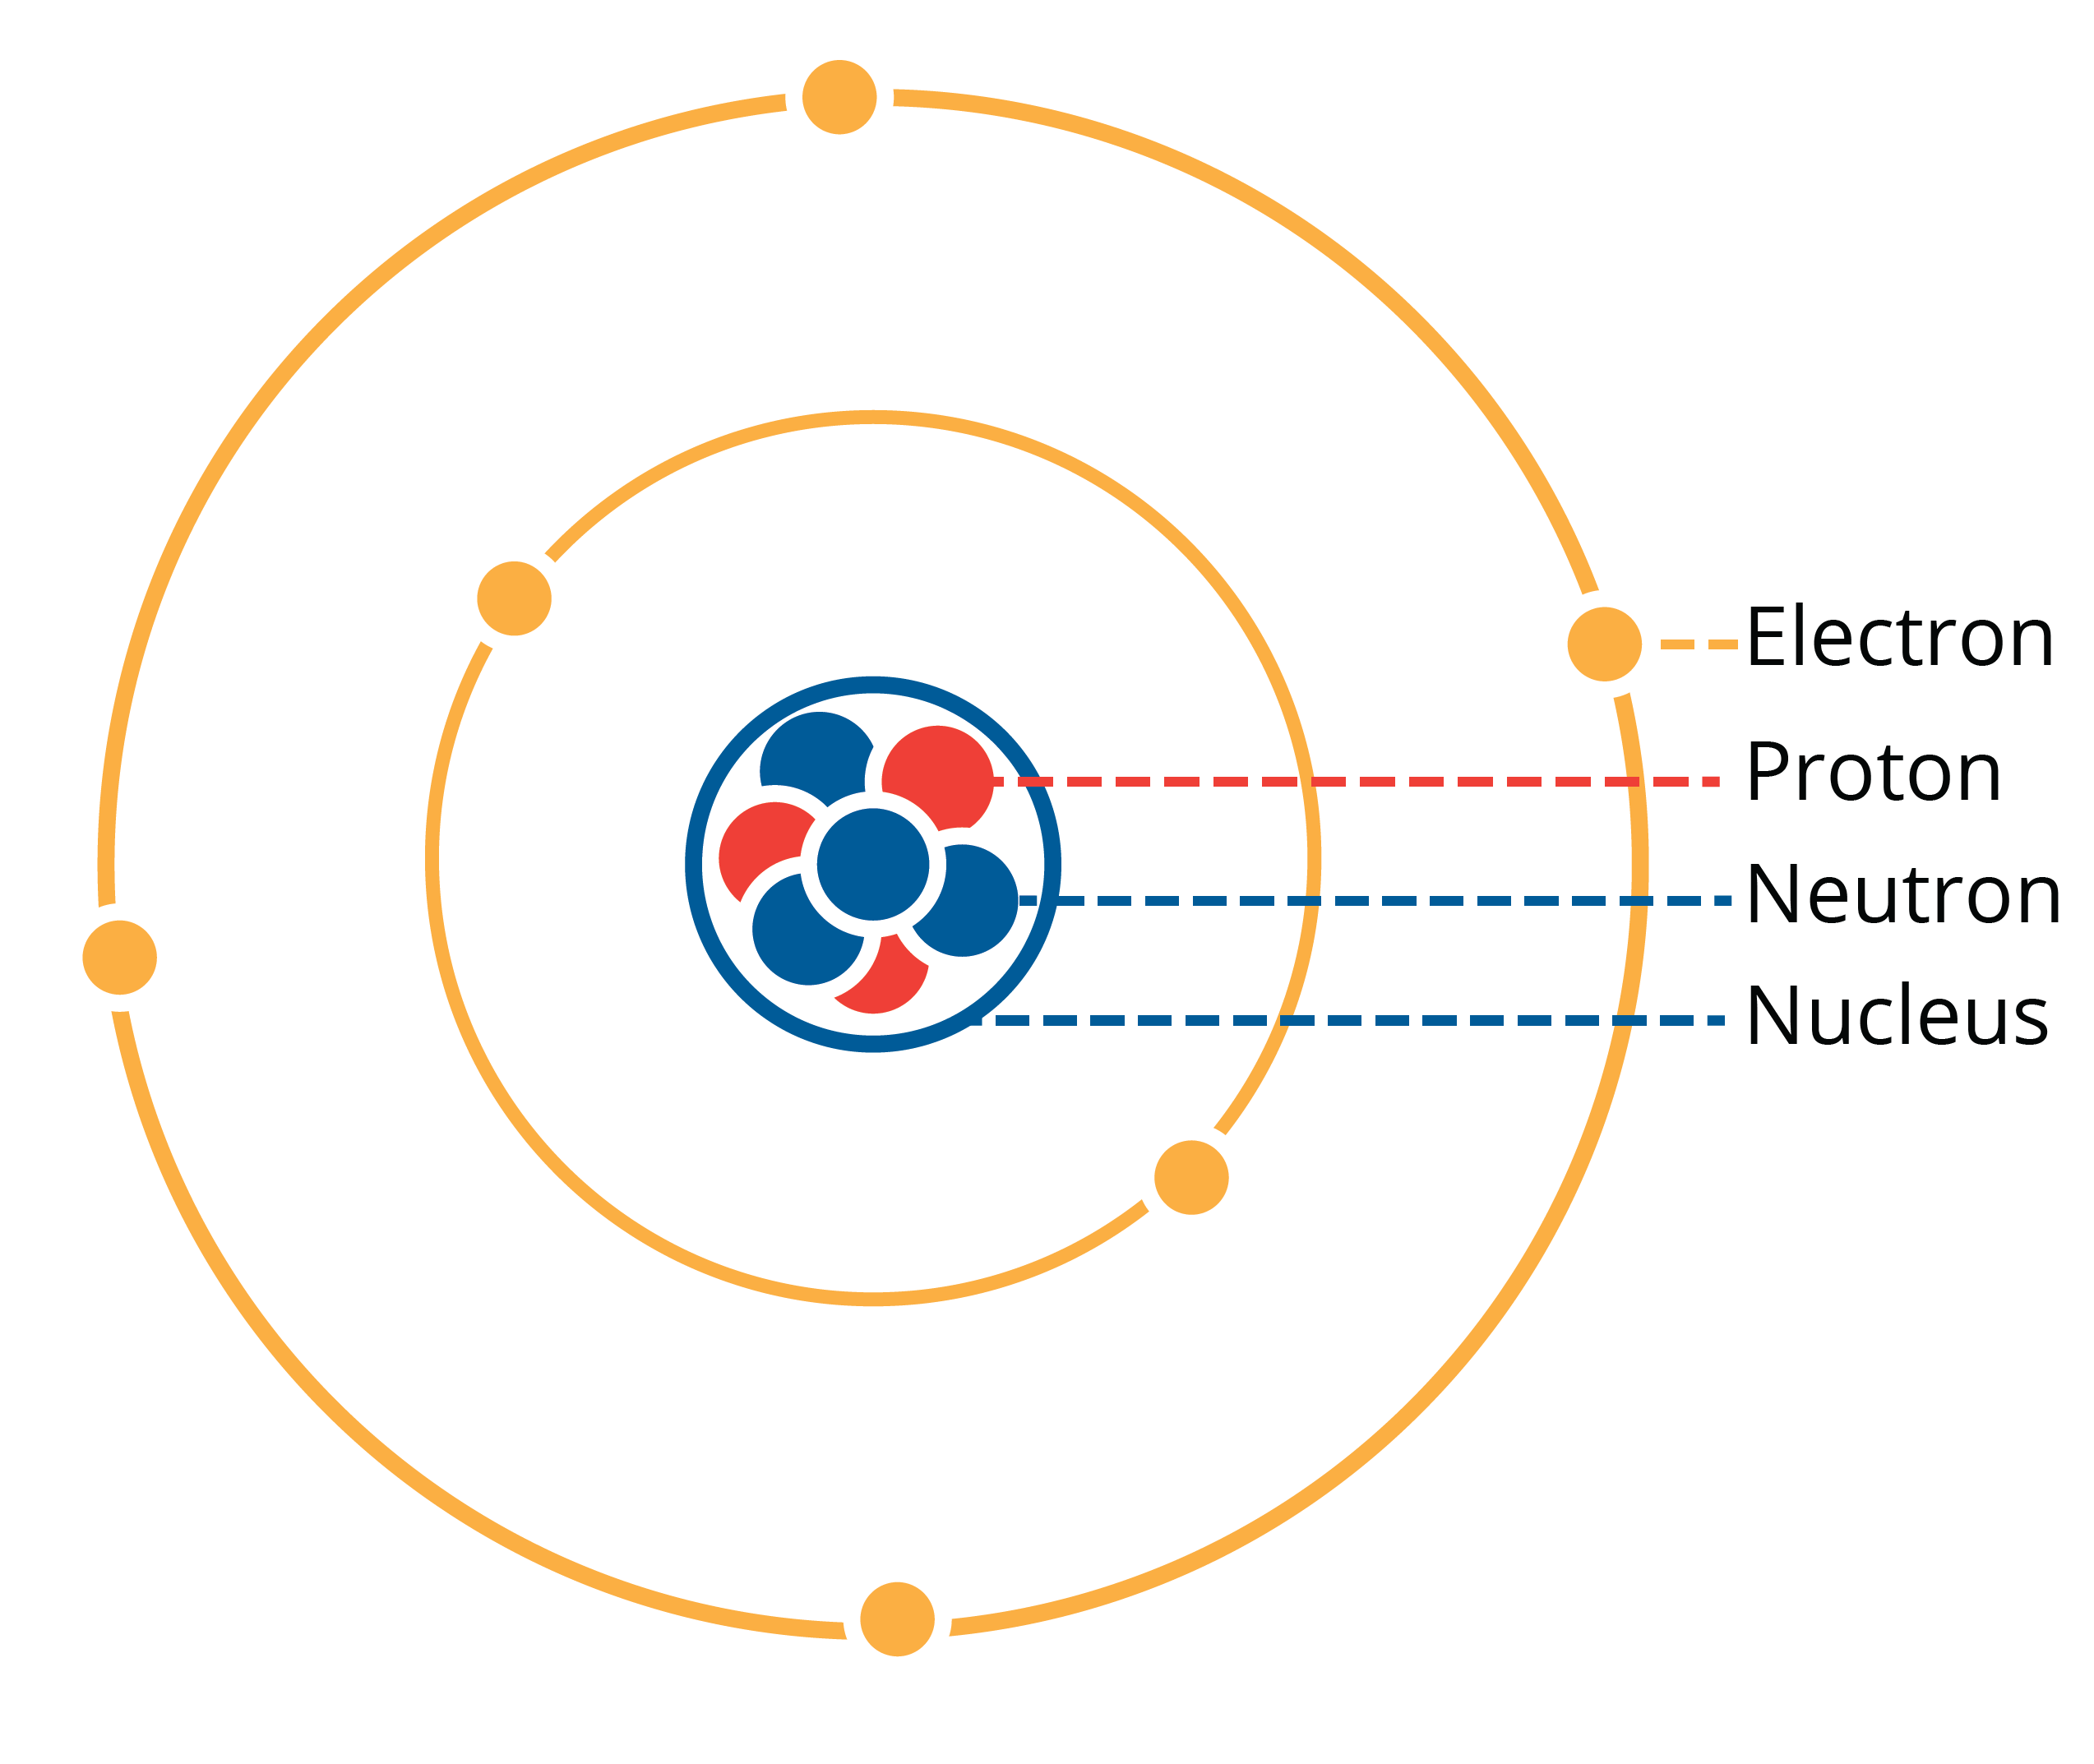
\includegraphics[width=2.5in]{atom1.png}
\caption{}
\label{fig:atom1}
\end{wrapfigure}

What is this ordinary matter made of? All things (including the air around you) 
are made of atoms. Atoms are incredibly tiny --- there are more atoms in a drop 
of water than there are drops of water in all the oceans.
% ADD: If you want a better visual of the scale: https://htwins.net/scale2/, start at around 10^-8

Every atom has a nucleus that contains protons and neutrons. Orbiting around the
nucleus is a cloud of electrons. However, the mass of the atom comes mainly from 
the protons and neutrons, since they are about 2000 times as massive as an 
electron! These three particles, protons, neutrons, and electrons, are called
\textit{subatomic particles}. (See figure \ref{fig:atom1}.) \index{protons} 
\index{neutrons} \index{electrons} \index{subatomic particle}

\section{Atoms and Their Models}
\begin{wrapfigure}{l}{3in}
\noindent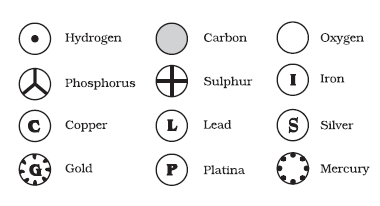
\includegraphics[width=2.5in, trim={0 0.5cm 0 0.5cm}, clip=true]{daltons_model.png}
\caption{}
\end{wrapfigure}

Over the history of science, there have been many ideas about the structure of
atoms. This history is a good example of how science develops: unexpected
results drive scientists to update their models, moving us closer and closer to
a true model of the atom.

During his investigations into the behavior of gases, John Dalton noted that 
different elements combine in strict ratios. For example, he noted that nitrogen 
and oxygen combine in a 1:1 and 1:2 fashion, but no ratio in between.

This first model of the atom is rudimentary; each element is a unique atom,
and those atoms cannot be subdivided. The atom is modeled as one large, solid,
uniform, and neutral object. British physicist J.J. Thomson discovered that
atoms could be split into a light, negatively charged particle and a heavier,
positively charged particle (we now know this is the nucleus, the dense
grouping of protons and neutrons in the center of an atom).

Suddenly, the atom went from neutral and indivisible to made of different types
of charged particles. Further experiments by Ernest Rutherford showed the atom
to be mainly empty space, further updating scientists' model of the atom.
Subsequently, Bohr explained the phenomena of spectral lines (we will discuss
this further in Sequence 2) by modeling electrons as being restricted to
orbiting specific distances from the nucleus.

\begin{wrapfigure}{l}{2in}
\noindent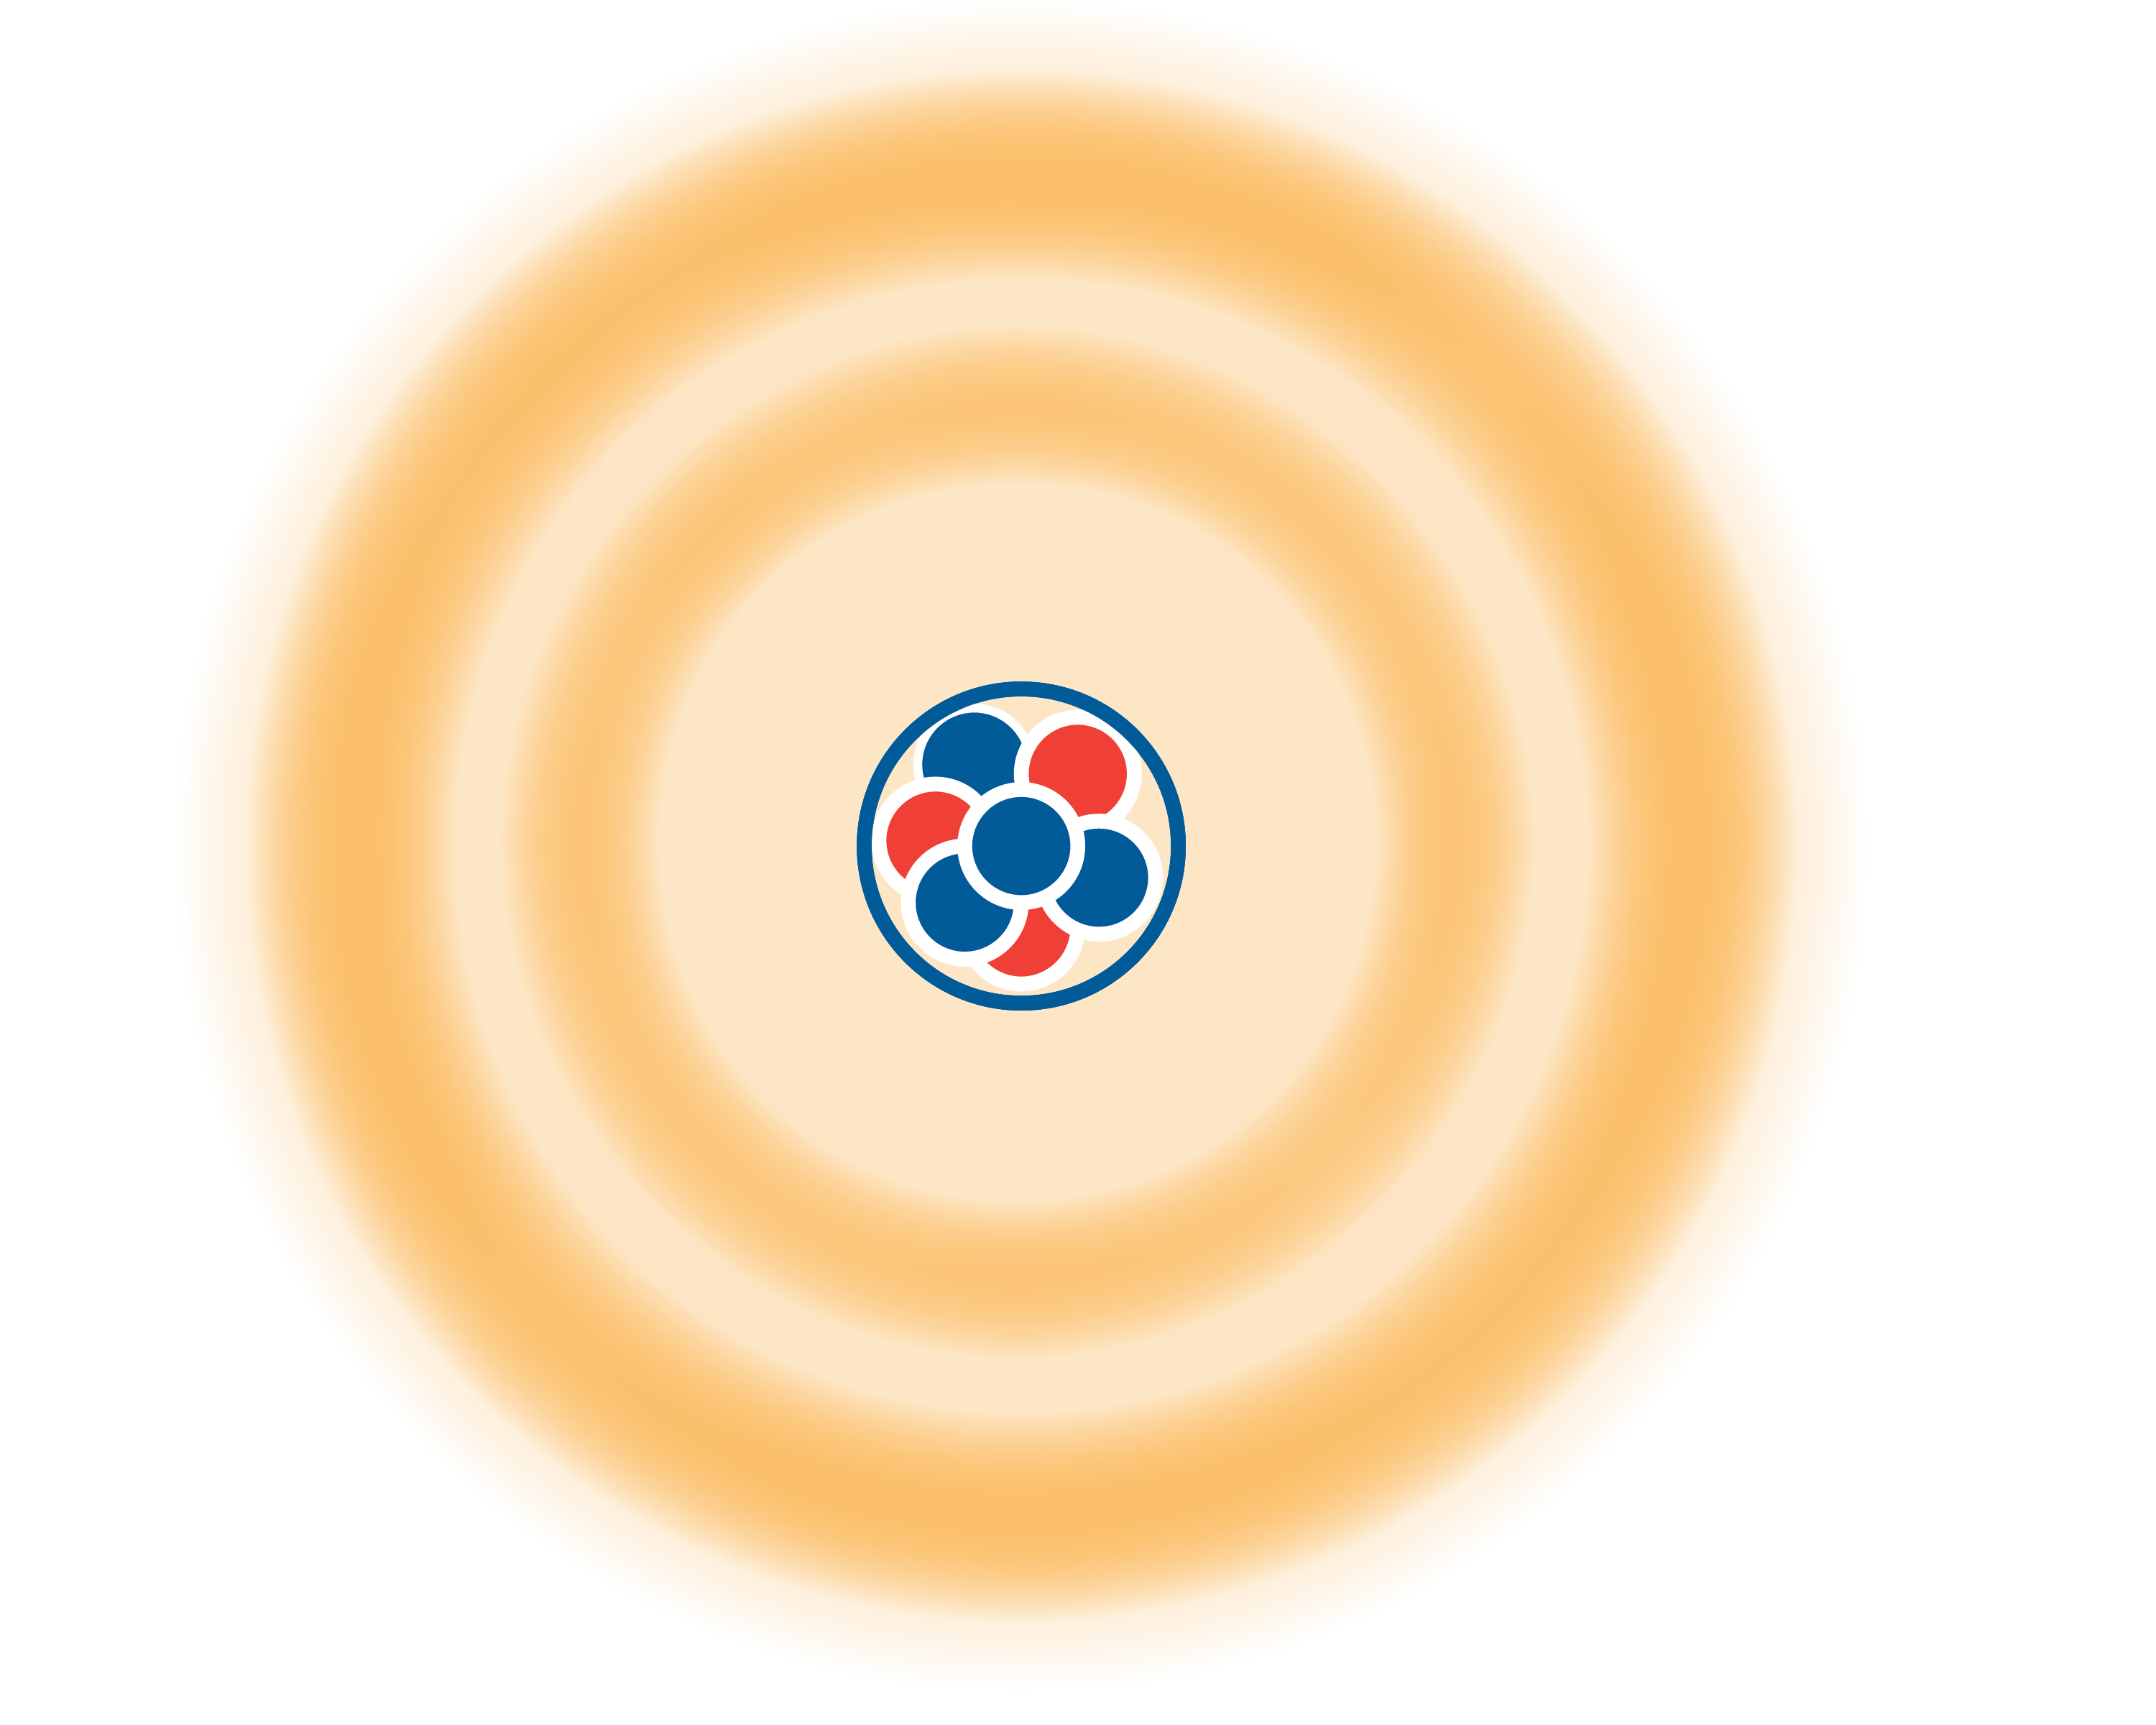
\includegraphics[width=2in]{atomCloud.png}
\caption{}
\label{fig:atomCloud}
\end{wrapfigure}

This is likely the model you are most familiar with seeing, and it is the one we
will use most often in this text. The first figure shown in this chapter is a Bohr
model: it shows the protons and neutrons in the nucleus, and models the electrons 
as moving in discrete orbits around the nucleus. 

However, the Bohr model is slightly inaccurate. While it is a convenient model for
thinking about atoms, in reality, electrons don't neatly orbit the nucleus.
Scientists don't know exactly where an electron will be in relation to the
nucleus, but they do know where it is most likely to be. They use a cloud that is
thicker in the center but fades out at the edges to represent an electron's
position (see figure \ref{fig:atomCloud}).

While the cloud model is more accurate, we will use the Bohr model as it
allows the viewer to easily and quickly assess the number and arrangement of
electrons.


\subsection{Classifying Atoms}
\begin{wrapfigure}{r}{2.5in}
    \centering
    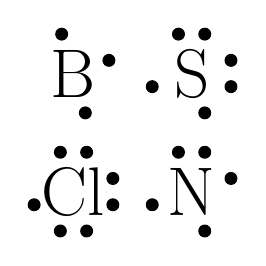
\begin{tikzpicture}
        \node[font=\Huge] at (-0.75,0) {B};
        \draw[fill=black] (-0.9, 0.5) circle (0.75mm);
        \draw[fill=black] (-0.3, 0.167) circle (0.75mm);
        \draw[fill=black] (-0.6, -0.5) circle (0.75mm);
        
        \node[font=\Huge] at (0.75, 0) {S};
        \draw[fill=black] (0.583, 0.5) circle (0.75mm);
        \draw[fill=black] (0.917, 0.5) circle (0.75mm);
        \draw[fill=black] (1.25, 0.167) circle (0.75mm);
        \draw[fill=black] (1.25, -0.167) circle (0.75mm);
        \draw[fill=black] (0.917, -0.5) circle (0.75mm);
        \draw[fill=black] (0.25, -0.167) circle (0.75mm);
        
        \node[font=\Huge] at (-0.75, -1.5) {Cl};
        \draw[fill=black] (-0.917, -1) circle (0.75mm);
        \draw[fill=black] (-0.583, -1) circle (0.75mm);
        \draw[fill=black] (-0.25, -1.333) circle (0.75mm);
        \draw[fill=black] (-0.25, -1.667) circle (0.75mm);
        \draw[fill=black] (-0.583, -2) circle (0.75mm);
        \draw[fill=black] (-0.917, -2) circle (0.75mm);
        \draw[fill=black] (-1.25, -1.667) circle (0.75mm);
        
        \node[font=\Huge] at (0.75, -1.5) {N};
        \draw[fill=black] (0.583, -1) circle (0.75mm);
        \draw[fill=black] (0.917, -1) circle (0.75mm);
        \draw[fill=black] (1.25, -1.333) circle (0.75mm);
        \draw[fill=black] (0.917, -2) circle (0.75mm);
        \draw[fill=black] (0.25, -1.667) circle (0.75mm);
    \end{tikzpicture}
    \caption{}
    \label{fig:Lewis_dot}
\end{wrapfigure}

We classify atoms by the numbers of protons they have. An atom with one proton
is a hydrogen atom, an atom with two protons is a helium atom, and so forth
(refer to Table~\ref{fig:periodic_tbl} on page~\pageref{fig:periodic_tbl})). We say that hydrogen and helium are \textit{
elements} because the classification of elements is based on the proton number.
And we give each element an atomic symbol. Hydrogen gets $H$, helium gets $He$,
oxygen gets $O$, carbon gets $C$\index{elements}, and so on. You can see an element's 
symbol on the periodic table. 


\subsection{When Atoms Combine}
When atoms of different elements combine, they make \textit{compounds}. Compounds
are substances made up of more than one element. Compounds can be 
\textit{molecules} or \textit{crystal lattices}. In the next section you'll learn
\textit{why} these different structures form. 

There are many kinds of compounds. You know a few:
\begin{itemize}
\item Table salt is crystals made of $Na^{+}$ and $Cl^{-}$ ions: a sodium atom 
that as lost an electron and a chlorine atom that gained an electron
\item Baking soda, or sodium bicarbonate, is $NaHCO_3$.
\item $O_2$ is the oxygen molecules that you breathe out of the air (air, a
blend of gases, is mostly $N_2$.).
\item Common quartz is $SiO_2$: silicon dioxide
\end{itemize}

The subscripts indicate what ratio of the elements are present in the compound. 
Each number indicates the ratio for the preceding element. A drop of water, 
$H_2O$, has twice as many hydrogen atoms as oxygen atoms. 

\textbf{Example}: What is the ratio of elements present in Epsom salt?

\textbf{Solution}: Epsom salt, chemical name magnesium sulfate, has the chemical formula $MgSO_4$. Therefore, the ratio of Mg:S:O is 1:1:4. 

\begin{Exercise}[title = {Ratios of Atoms in Molecules}, label = num_atom]
Give the elemental ratio for each compound. 
\begin{enumerate}
\item methane, $CH_4$
\item copper (II) sulfate, $CuSO_4$
\item glucose, $C_6H_{12}O_6$
\end{enumerate}
\end{Exercise}

\begin{Answer}[ref = num_atom]
\begin{enumerate}
\item C:H = 1:4
\item Cu:S:O = 1:1:4
\item C:H:O = 6:12:6 = 1:2:1
\end{enumerate}
\end{Answer}

\section{Types of Matter}
One way to classify matter is by the types of chemical bonds that hold a 
material's atoms together. The nature of these bonds, in turn, affects the 
properties of the material. For now, all you need to know is there are three types
of chemical bonds: metallic, covalent, and ionic. Materials held together with the
same type of bonds tend to have similar properties. For example, copper, bronze, 
iron, and steel (all containing metallic bonds) are all shiny, ductile, malleable,
and good conductors of heat and electricity. On the other hand, Epsom salt and 
table salt form large crystals, have very high melting points, and are poor 
conductors of electricity in their pure form. These two substances (Epsom and 
table salt) both contain ionic bonds. 

\subsection{Covalent Compounds}
Water is an example of a covalent compound: it is made of two hydrogen atoms 
covalently bonded one oxygen atom (see figure \ref{fig:water_polar}). The result 
is a water molecule\index{molecules}. The different atoms cluster together 
because they share electrons in their clouds. This is the nature of a 
\textit{covalent bond}\index{covalent bond}: it is formed when atoms share electrons.
Sometimes, electrons are shared evenly, but in water, they are shared unevenly. 
Oxygen is better at attracting electrons to itself than hydrogen, and so the 
shared electrons  so they spend more time on the oxygen atom than the hydrogen 
atoms. As a result, the oxygen side of a water molecule has a slight negative 
charge, while the hydrogen atoms have a slight positive charge. These slight 
charges are represented with a lower case Greek letter delta, $\delta$. When 
electrons are shared unevenly, we call this a \textit{polar} covalent bond, 
because there are positive and negative poles at either end of the bond. 
\index{polar bond} \index{non-polar bond}

\begin{wrapfigure}{r}{3.25in}
\noindent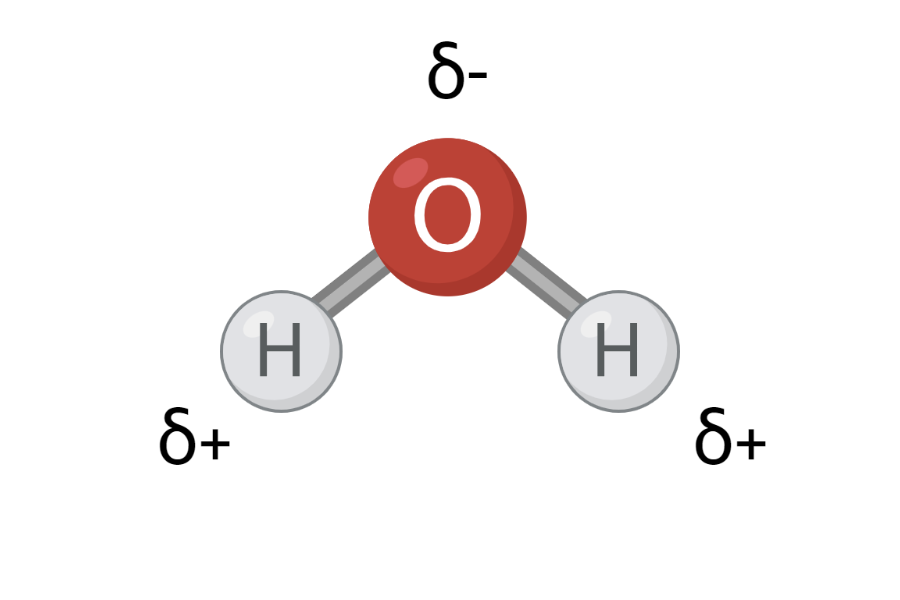
\includegraphics[width=3.25in]{water_polar.png}
\caption{}
\label{fig:water_polar}
\end{wrapfigure}

Whether electrons are shared evenly or unevenly is based on the elements' relative 
\textit{electronegativities}.\index{electronegativity} Electronegativity is simply
a measure of how strongly an atom can attract electrons to itself. In general, 
elements on the right side of the periodic table are more electronegative than 
elements on the left side. When covalent bonds form between two elements of similar electronegativities, the electrons are shared evenly. We call this a \textit{non-polar}
covalent bond. Oil is an example of a non-polar covalent substance. Different 
oils have different ratios and structures, but all oils are made mainly of carbon 
and hydrogen, which have similar electronegativities. What happens when you try to 
mix oil and water? They don't mix well! This is due to the difference between 
their bond types. Polar substances, like water, mix best with other polar 
substances, while non-polar substances, like oils, mix best with non-polar 
substances. You'll learn more about why this is in Sequence 2.

For both polar and non-polar covalent bonds, the electrons are held tightly to 
the nuclei, even if they are shared among atoms. Those electrons don't move to 
another molecule: they move around within the molecule they are already a part 
of. Since electrons don't flow freely in covalent substances, they are also poor 
conductors of electricity. Covalent compounds also tend to have lower melting and 
boiling points compared to ionic compounds. 

\subsection{Ionic Compounds}
\begin{wrapfigure}{l}{3in}
\noindent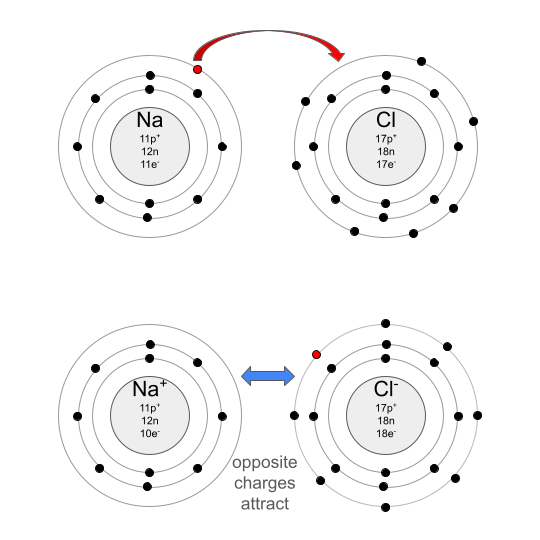
\includegraphics[width=3in]{NaCl_xfer.png}
\caption{}
\label{fig:NaCl_xfer}
\end{wrapfigure}
Ionic bonds are the electrical attraction between opposite-charged ions. When a 
neutral atom gains or loses an electron it becomes an \textit{ion} (a charged 
atom), and oppositely-charged ions are attracted to each other. Which atom gets 
the electron and which loses it is based on their electronegativities: the more 
electronegative atom steals one or more electrons from the less electronegative 
atom. There are also polyatomic ions: groups of atoms held together with covalent 
bonds that have an overall charge (figure ... shows the Lewis dot structure of a phosphate polyatomic ion, as an example). For now, we'll focus just on 
ionic bonds between monoatomic ions, like in table salt. You'll learn more about 
polyatomic ions and the compounds they form in Sequence 2. 

Let's examine how a simple ionic compound is formed: sodium chloride, also known 
as table salt, is made up of sodium and chlorine atoms (see figure 
\ref{fig:NaCl_xfer}). When sodium and chlorine come in contact with each other, 
electrons move from the sodium to the chlorine, making a sodium \textit{cation} 
(positively-charged ion) and a chloride \textit{anion} (negatively-charged ion). 
Yes --- chlor\textit{ide} is correct! When naming an anion, the ending of the 
element name changes to \textit{-ide}. Once the sodium cation and chloride anion 
are formed, their opposite charges attract them to each other, like north and 
south magnet poles. 

\begin{wrapfigure}{l}{2in}
\noindent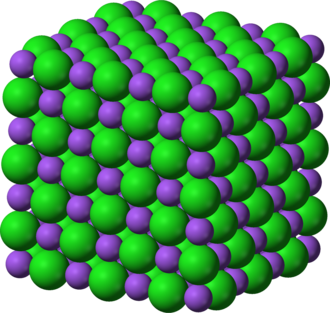
\includegraphics[width=2in]{NaCl_lattice.png}
\caption{}
\label{fig:NaCl_lattice}
\end{wrapfigure}

When there are many, many sodium and chloride ions around, they spontaneously 
arrange themselves in a pattern, giving ionic compounds their characteristic 
crystal structure (see figure \ref{fig:NaCl_lattice}). Because the electrons are 
tightly held be each ion, ionic substances don't conduct electricity well as 
solids. The atomic crystal lattice also determines the shape of the macroscopic 
crystals. Salt crystals are generally cubic, while other crystals (like quartz) 
form hexagonal prisms. You'll learn how to predict the atomic and macroscopic 
crystal structure of different compounds in Sequence 2. 

<<<<<<< HEAD
=======
\subsubsection{Modeling Ionic Compounds}
You can represent ions with Lewis dot diagrams by adding or subtracting electrons 
from the model. Since electrons are negative, anions have gained electrons while 
cations have lost them. Additionally, the ion is in brackets and the overall 
charge is indicated outside the top right corner of the brackets. 

\textbf{Example}: Create Lewis dot diagrams for $\text{Na}^{+}$, $\text{F}^{-}$, 
$\text{O}^{2+}$, and $\text{Mg}^{-}$.

\textbf{Solution}: Sodium is in column 1, so a neutral sodium atom has 1 valence 
electron. A +1 charge means it has lost 1 electron, leaving zero.

\begin{center}
    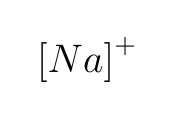
\begin{tikzpicture}
        \node[font = \Large] at (0,0) {$\left[ \text{Na} \right]^{+}$};
     \end{tikzpicture}
\end{center}

Fluorine is in column 17 and has 7 valence electrons when neutral. The anion 
$\text{F}^-$ has gained one electron, for a total of 8. 

\begin{center}
    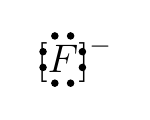
\begin{tikzpicture}
        \node[font = \Large] at (0,0) {$\left[ \text{ F } \right]^-$};
        \draw[fill=black] (-0.4, 0.1) circle (0.4mm);
        \draw[fill=black] (-0.4, -0.1) circle (0.4mm);
        \draw[fill=black] (0.1, 0.1) circle (0.4mm);
        \draw[fill=black] (0.1, -0.1) circle (0.4mm);
        \draw[fill=black] (-0.05, 0.3) circle (0.4mm);
        \draw[fill=black] (-0.25, 0.3) circle (0.4mm);
        \draw[fill=black] (-0.05, -0.3) circle (0.4mm);
        \draw[fill=black] (-0.25, -0.3) circle (0.4mm);
    \end{tikzpicture}
\end{center}

Neutral oxygen has 6 valence electrons, therefore $\text{O}^{2+}$ has 4. 
\begin{center}
    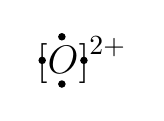
\begin{tikzpicture}
        \node[font = \Large] at (0,0) {$\left[ \text{ O } \right]^{2+}$};
        \draw[fill=black] (-0.5, 0) circle (0.4mm);
        \draw[fill=black] (0.03, 0) circle (0.4mm);
        \draw[fill=black] (-0.25, 0.3) circle (0.4mm);
        \draw[fill=black] (-0.25, -0.3) circle (0.4mm);
    \end{tikzpicture}
\end{center}

Neutral magnesium has 2 valence electrons, so $\text{Mg}^{-}$ has 3 valence 
electrons. 
\begin{center}
    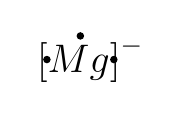
\begin{tikzpicture}
        \node[font = \Large] at (0,0) {$\left[ \text{ Mg } \right]^{-}$};
        \draw[fill=black] (-0.55, 0) circle (0.4mm);
        \draw[fill=black] (0.3, 0) circle (0.4mm);
        \draw[fill=black] (-0.125, 0.3) circle (0.4mm);
    \end{tikzpicture}
\end{center}

To make Lewis dot diagrams of ionic compounds, you show both ions in the ratio 
given in the formula. For example, a Lewis dot diagram of $\text{MgCl}_2$ would 
show one magnesium cation and two chloride anions. 

>>>>>>> dbf2f61febb5038df393d9df265d14e215d8c7c0
\subsection{Metallic Compounds}
You may already know that metals (both pure and alloyed) are excellent conductors 
of electricity and heat. This is a consequence of their metallic bonds. In pure 
metals and alloys, the outermost layer of electrons can move freely from one atom 
to the next. As a result, at the atomic level, metals are best characterized as a 
lattice of cations surrounded by a ''sea of electrons" (see figure	fixme metallic bonding figure)

The free-flowing sea of electrons in pure and alloyed metal means the cation 
lattice can be rearranged without breaking the metallic bond. As a result, metals 
are ductile (able to be drawn out into a wire) and malleable (able to be hammered 
into a new shape without cracking or breaking). (fixme figure showing deformation of cation lattice in bending metal)

Metals can be pure, like copper or iron, or \textit{alloys}, like bronze or steel. 
\textit{Alloys} are mixtures between two or more elements where at least one 
element is a metal.\index{alloy} Steel is an alloy of iron and carbon; bronze is 
an alloy of copper and tin. Alloying a metal changes its properties because of 
the change in the cation lattice (see figure fixme pure vs alloyed lattice and 
structural changes). 

\section{Energy and Work}

Energy is defined as the ability to do work, but what does this mean? First, we 
need to understand what \textit{work} is. When you lift an object into the air, 
you are doing work on that object. When water turns a turbine in a hydroelectric 
plant, the water is doing work on the turbine. And when you hit the brakes on your
car, the brake pads are doing work on the tires (albeit, negative work). 
\textit{Energy} is being transferred between these pairs of objects when work is 
done. 

Some everyday examples of energy include:
\begin{enumerate}
\item The Calories in your food
\item The light from the Sun
\item Heat in the Earth's mantle
\item The motion of a spinning wheel
\end{enumerate}

Some types of energy are easy to visualize, while others are not. Energy is what 
moves from one object to another when work is being done. When you lift 
something, the energy stored in your body (in the form of sugar and fat) is 
transferred to the object, accelerating it upwards. Your body continues to 
transfer energy as you lift the object against gravity. When you've lifted it as 
high as you can, most of the energy your body lost (we call this "burning 
Calories" colloquially) is stored as \textit{potential energy}, due to the 
object's height. 

Another example is a simple circuit connecting a battery and a light bulb. The 
battery has stored potential energy. When the circuit is complete, the potential 
energy in the battery is transferred to electrons in the light bulb, causing them 
to move and gain kinetic energy. In the light bulb's filament (we are referencing 
old, non-LED light bulbs here!), the electrons encounter resistance, which slows 
them down. The energy the electrons lose in this process is being transformed into 
light and heat, lighting your room. 

The Work-Energy theorem explains the relationship between work and energy, and we 
will introduce the theorem and use it to explain energy transfer in a subsequent 
chapter. 

\section{Mass-Energy Equivalence}
You've probably seen the equation
$$E = mc^2$$

$E$ is energy, $m$ is mass, and $c$ is the speed of light in a vacuum (about $3 
\times 10^8 \frac{m}{s}$). So far, we've been discussing matter and energy 
separately. This equation shows that matter can be converted to energy, and 
vice-versa. This is the source of the light energy emitted by the sun. 

The Sun is mostly hydrogen. At the very center, it is so hot and dense that the 
nuclei of hydrogen atoms are fused together to form helium atoms, a process 
called the proton-proton chain reaction. The actual reaction involves several 
steps and is more complicated, but the overall process can be summarized as:

$$4\text{H} \to \text{He}$$

If every hydrogen atom has a mass of approximately $1.6735575 \times 10^{-27}$ kg 
and every helium atom has a mass of approximately $6.6464731 \times 10^{-27}$ kg, 
how much energy is released when one atom of helium is created? First, notice 
that one helium has less mass than 4 hydrogen atoms:

$$4 \times \left( 1.6735575 \times 1-^{27} \right) - 6.6464731 \times 10^{-27} = 
4.77569 \times 10^{-29}$$

Now, we can use $E = mc^2$ to find out how much energy is equivalent to $4.77569 
\times 10^{-29}$ kg:

$$E = \left( 4.77569 \times 10^{-29} \text{kg} \right) \left( 2.99792458 \times 
10^8 \frac{\text{m}}{\text{s}} \right)^2$$
$$E \approx 4.292 \times 10^{-12} \text{joules}$$

All of these numbers are very small and hard to visualize. We could ask this: if 
1 kilogram of hydrogen (about enough to fill a standard beach ball) were fused to 
make helium, how much energy would be released? For every kilogram of hydrogen 
that enters the proton-proton chain reaction, about 0.02854 kilograms of mass are 
converted to energy (the mass of about 5 quarters).

$$E = \left( 0.02854 \text{ kg} \right) \left( 2.99792458 \times 10^8 \frac{
\text{m}}{\text{s}} \right)^2 \approx 2.5647 \times 10^{15} \text{ joules}$$

This is more than 700,000,000 kWh (kilowatt hours); the average US household 
uses only 30 kWh per day. Fusing one kilogram of hydrogen releases enough energy 
to power an average US home every day for \textit{over 65,000 years}! This 
relatively huge release of energy is why scientists continue to research nuclear 
fusion energy sources. The nuclear power plants currently running around the world 
today rely on \textit{nuclear fission}: the splitting apart of atoms, the opposite 
process of \textit{nuclear fusion}. Nuclear fission releases much, much less energy 
per kilogram of input material than nuclear fusion, and thus stable, affordable 
nuclear fusion power plants remain a ''holy grail" of scientific research. 

\section{Conclusion}
We have seen that the universe is made of dark energy, dark matter, and ordinary matter. Ordinary matter is made of atoms, which can be classified based on their number of protons. Atoms combine in different ways to make compounds, and the manner of combination (ionic, covalent, or metallic bonding) affects the macroscopic properties of the substance. Energy allows matter to do work, and work is the transfer of energy. 

Matter and energy do share a fundamental property: they are both conserved. Neither matter nor energy can be created or destroyed. This means the total amount of ordinary matter and energy in the universe is constant. This great scientific truth *something about its application* In the next chapter, 
%FIXME cliffhanger on above sentence







%FIXME Global layout note: Let's discuss adding Title's and Captions to all graphics.\\

%For example:\\
%TITLE: Mass versus Weight\\
%CAPTION: Human Earth weight: 150lbs / Moon weight:??lbs\\
%Potato Earth weight: .25lbs / Moon weight: ??lbs \\

%FIXME:
%Allison thinks it would be funny if the person in the graphic were holding a potato and we also added the weight and mass of the potato to the caption. No worries if this type of edit isn't in the budget!

%FIXME: What are your thoughts about using the metric system consistently -- in which case we'll replace pounds here with kilos. Max notes: we should explicitly use kilos for mass and pounds or newtons for weight. Kilos are a scalar measure of the amount of matter and pounds are a vector force of gravity on a particular piece of matter. Many students struggle to differentiate between mass and weight at a theoretical level due to casual comparison between pounds and kilos.
